% Designed by Yiming Xu and Xiangjian Zhang in Gainesville, FL.
% All rights reserved.

% Excel to Latex: https://www.tablesgenerator.com/

\documentclass[final]{beamer}

% ====================
% Packages
% ====================

\usepackage[flushleft]{threeparttable}
\usepackage[T1]{fontenc}
\usepackage{lmodern}
\usepackage[size=custom,width=120,height=72,scale=1.0]{beamerposter}
\usetheme{gemini}
\usecolortheme{uchicago}
\usepackage{graphicx}
\usepackage{booktabs}
\usepackage{tikz}
\usetikzlibrary{arrows.meta}
\usepackage{pgfplots}
\pgfplotsset{compat=1.17}
\usepackage{caption}

\definecolor{posterblue}{RGB}{7,84,156}
\definecolor{posterorange}{RGB}{250,70,22}

% ====================
% Lengths
% ====================

% If you have N columns, choose \sepwidth and \colwidth such that
% (N+1)*\sepwidth + N*\colwidth = \paperwidth
\newlength{\sepwidth}
\newlength{\colwidth}
\setlength{\sepwidth}{0.025\paperwidth}
\setlength{\colwidth}{0.3\paperwidth}

\newcommand{\separatorcolumn}{\begin{column}{\sepwidth}\end{column}}

% ====================
% Title
% ====================

\title{E-bike, e-scooter, and bicycle crashes in Florida: evidence from LLM-classified crash narratives}

\author{Rithika Mathew \inst{1} {\normalsize (rmathew1@ufl.edu)} \and Yiheng Qian \inst{2} \and Xingjing Xu \inst{3} \and Ilir Bejleri \inst{3} \and Xiang 'Jacob' Yan \inst{2} {\normalsize (xiangyan@ufl.edu)}}

\institute[shortinst]{\inst{1} Department of Computer and Information Science and Engineering \samelineand \inst{2} Department of Civil and Coastal Engineering \samelineand \inst{3} Department of Urban and Regional Planning, University of Florida}


% ====================
% Footer (optional)
% ====================

\footercontent{
  \href{ }{ } \hfill
  Just \& Green Transportation Lab, University of Florida \hfill
  \href{}{}}
% (can be left out to remove footer)

% ====================
% Logo (optional)
% ====================

% use this to include logos on the left and/or right side of the header:
% \logoright{\includegraphics[height=7cm]{logo1.pdf}}
% \logoleft{\includegraphics[height=7cm]{logo2.pdf}}

% ====================
% Body
% ====================

\begin{document}
\addtobeamertemplate{headline}{}
{
    \begin{tikzpicture}[remember picture,overlay]
      \node [anchor=north west, inner sep=3cm] at ([xshift=1.2cm,yshift=-3cm]current page.north west)
      {\includegraphics[height=2.5cm]{logos/UFTransportation_Institute.png}}; % also try shield-white.eps
      \node [anchor=north east, inner sep=3cm] at ([xshift=-1cm,yshift=-2.6cm]current page.north east)
      {\includegraphics[height=2.8cm]{logos/logo.png}};
    \end{tikzpicture}
}

\begin{frame}[t]
\begin{columns}[t]
\separatorcolumn

\begin{column}{\colwidth}

  \begin{block}{Background}
  \begin{itemize}
      \item \textcolor{posterblue}{\textbf{E-bikes and e-scooters}} are the fastest-growing active modes in Florida, and crashes involving them are rising.
      \item Florida's crash report has \textcolor{posterblue}{\textbf{no field for an e-bike or an e-scooter}}. Both are coded as bicyclists, and the device appears only in the officer's \textcolor{posterblue}{\textbf{free-text narrative}}.
      \item Statewide statistics therefore \textcolor{posterblue}{\textbf{mix three modes}} with different riders and risks, a national gap noted by the NTSB (2022). Prior studies read \textcolor{posterblue}{\textbf{small, single-city samples}} by hand.
  \end{itemize}
  \end{block}

  \begin{block}{Research Objectives}
    \begin{itemize}
      \item Develop a \textcolor{posterblue}{\textbf{statute-grounded LLM framework}} that recovers e-bike, e-scooter, and bicycle crashes from narratives.
      \item Build an \textcolor{posterblue}{\textbf{interactive crash dashboard}} of Florida active-mode crashes, 2014--2026.
      \item Compare \textcolor{posterblue}{\textbf{riders, timing, location, severity, and causes}} across the three modes, and propose \textcolor{posterblue}{\textbf{countermeasures}}.
    \end{itemize}
  \end{block}

  \begin{block}{Data and Methodology}
Crash reports come from \textcolor{posterblue}{\textbf{Signal4 Analytics}} (FLHSMV), joined with FDOT roadway data. We hand-labeled \textcolor{posterblue}{\textbf{300 narratives}} using Florida Statute \S~316.003 (e-bike: pedals and a motor under 750~W; e-scooter: no pedals) and benchmarked five LLMs with the same few-shot prompt at temperature 0.

\begin{table}[!ht]\tiny%
\caption{LLM benchmark on 300 hand-labeled narratives}
\resizebox{.7\columnwidth}{!}{
\centering
\begin{tabular}{llc}
\hline
Model & Deployment & Accuracy \\ \hline
\textbf{Qwen2.5-72B (selected)} & Local, HiPerGator & \textbf{98.67\%} \\
Llama 3.1-70B & Local, HiPerGator & 98.67\% \\
Claude 3.7 Sonnet & API & 98.00\% \\
GPT-4o-mini & API & 93.00\% \\
DeepSeek-R1-14B & Local, HiPerGator & 92.95\% \\
\hline
\end{tabular}}
\end{table}

Multi-agent designs \textcolor{posterblue}{\textbf{did not beat}} the single best model. A second Qwen pass coded \textcolor{posterblue}{\textbf{rider location, cause, and fault}} for 18,562 narratives.

\begin{figure}
  \centering
  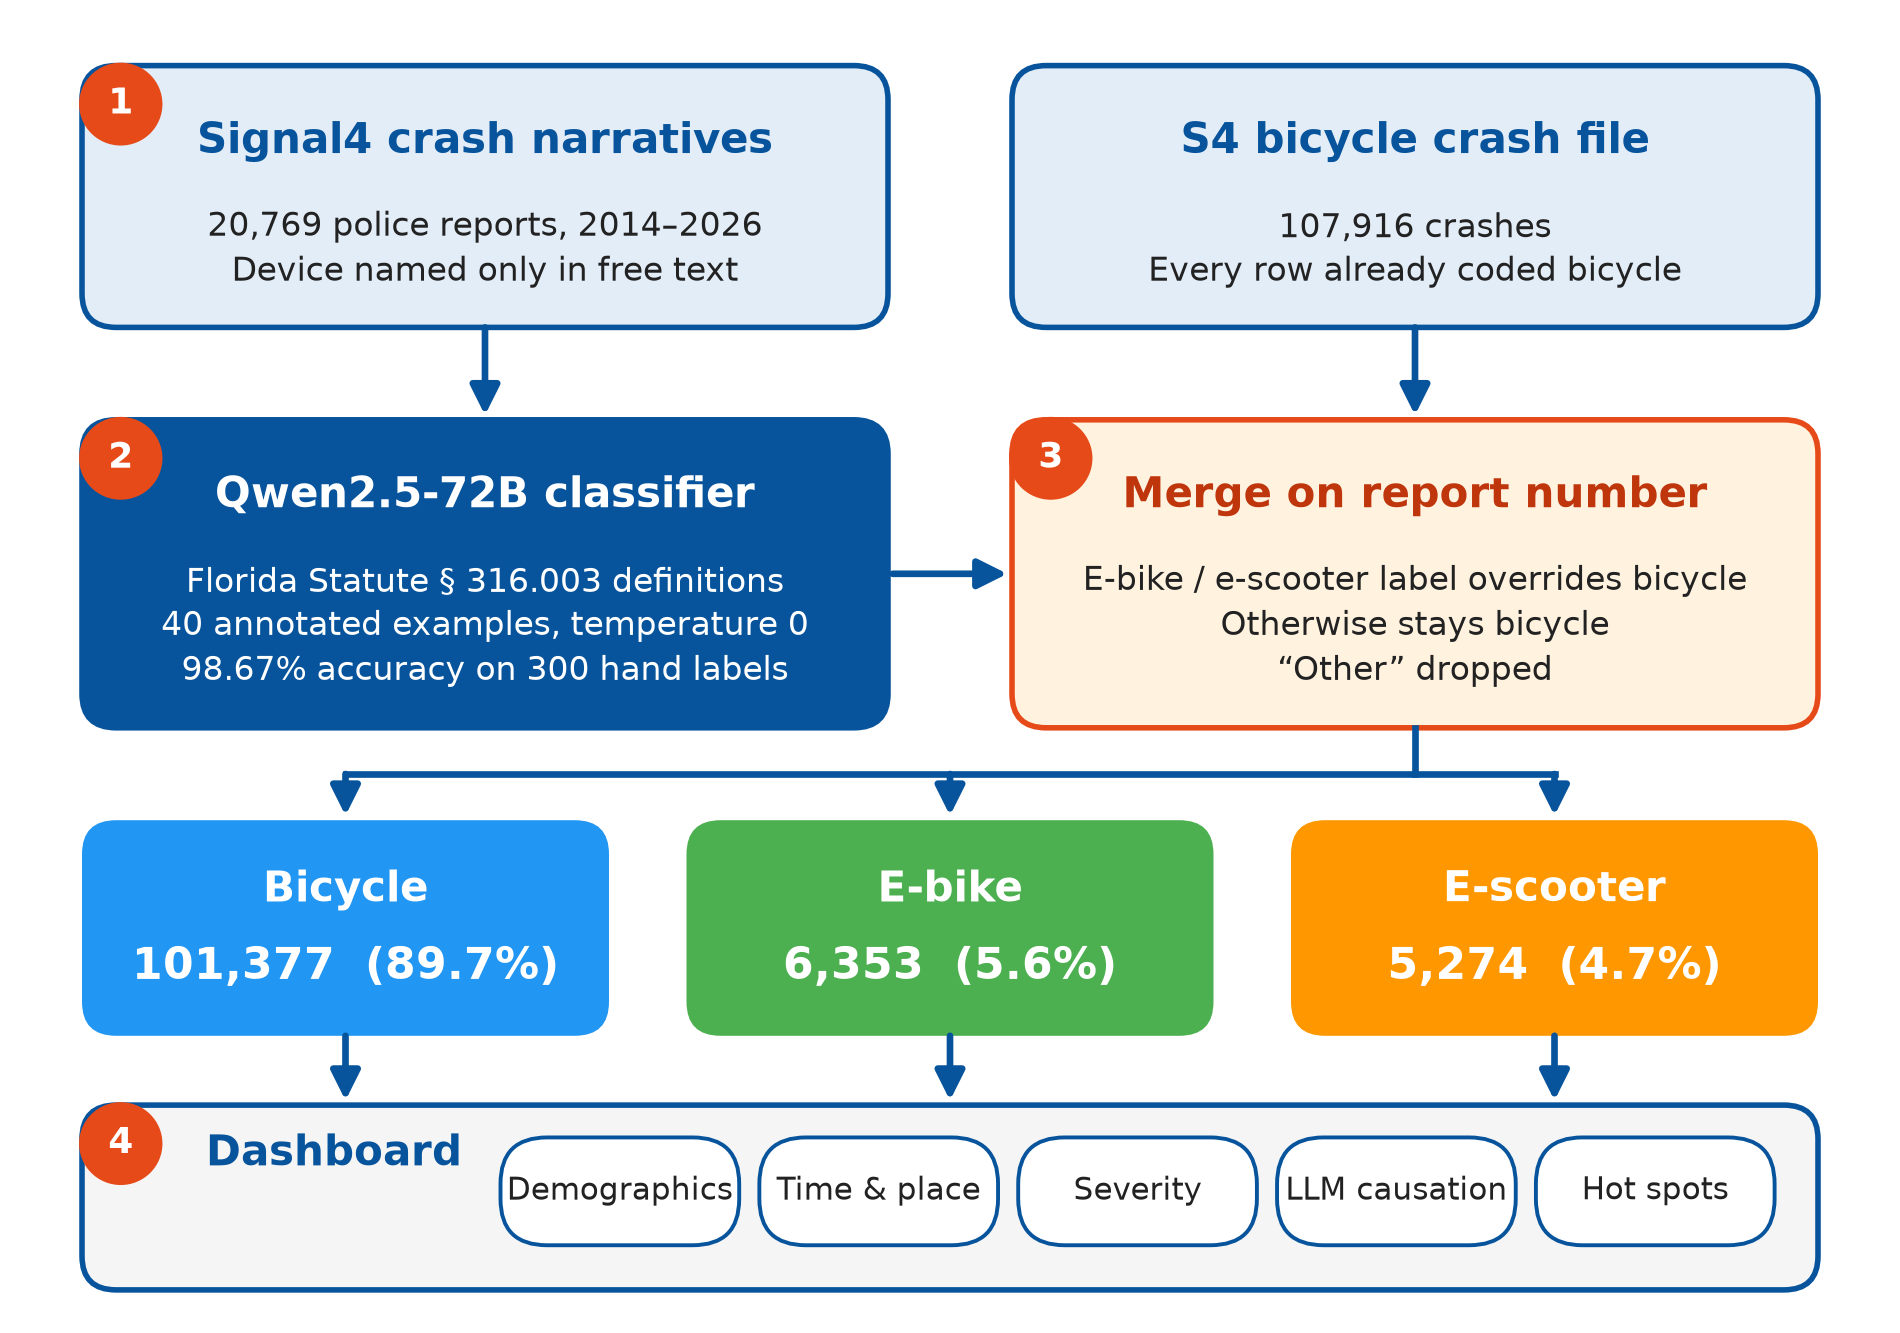
\includegraphics[width=0.95\linewidth,height=15.5cm,keepaspectratio]{figures/workflow.png}
  \caption{Classification and analysis workflow. E-bike and e-scooter counts are a floor: a crash is counted only if the narrative names the device.}
\end{figure}

  \end{block}

\end{column}

\separatorcolumn

\begin{column}{\colwidth}

\begin{figure}
  \centering
  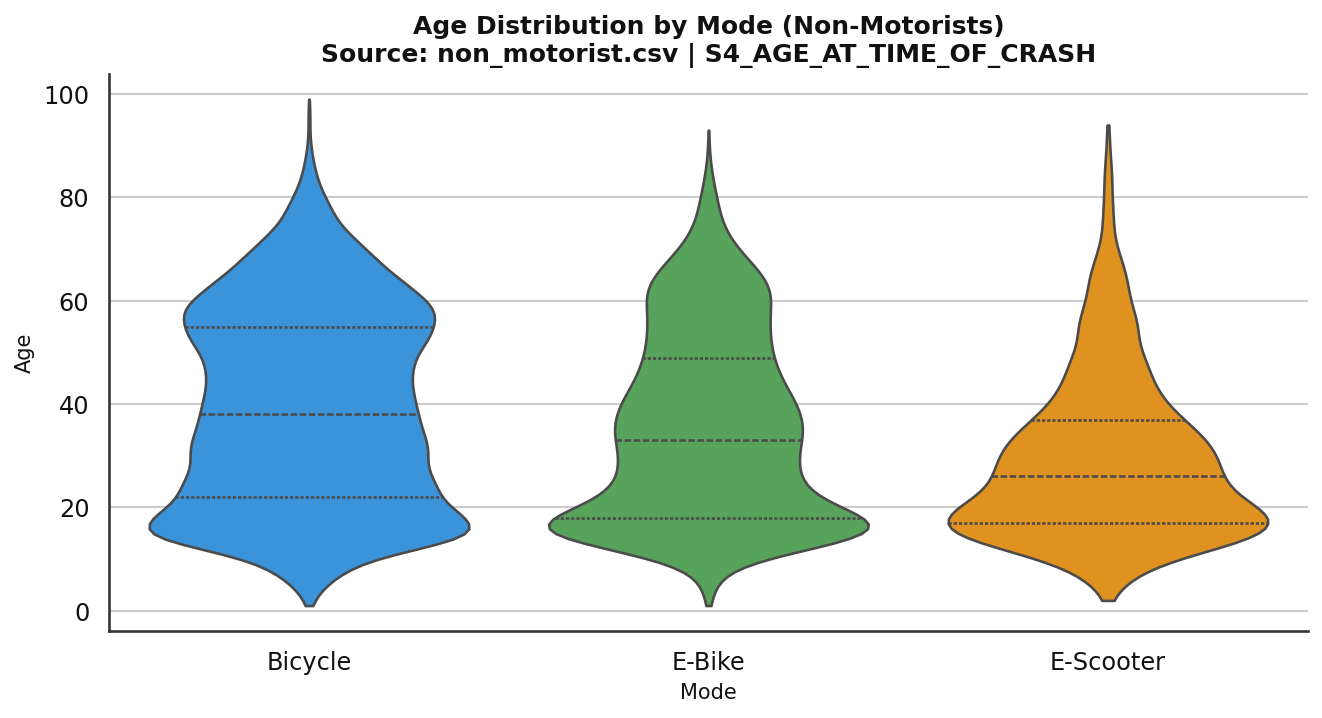
\includegraphics[width=0.49\linewidth,height=10cm,keepaspectratio]{figures/2a_age_violin.png}
  \hspace{0.01in}
  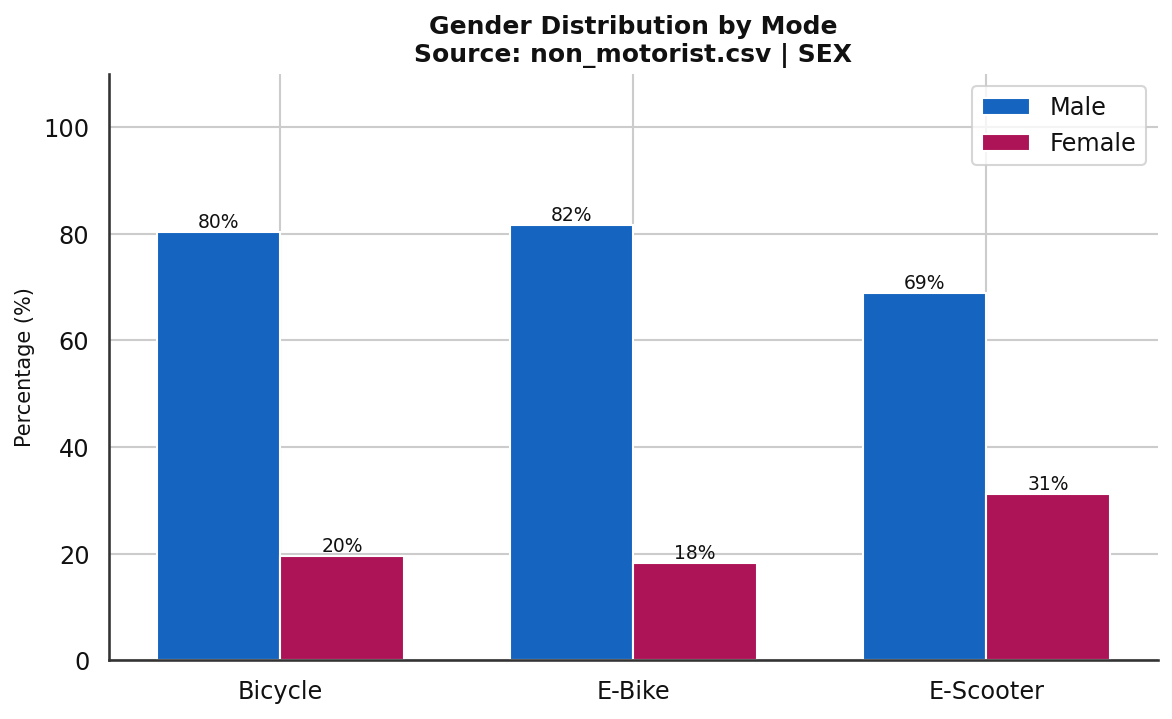
\includegraphics[width=0.49\linewidth,height=10cm,keepaspectratio]{figures/2c_gender_by_mode.png}
  \captionsetup{font={small,bf,stretch=1.25}}
  \caption{(a). Rider age by mode    (b). Rider sex by mode, among records with sex coded}
\end{figure}

  \begin{block}{Crash characteristics by mode}

\begin{table}[!ht]\tiny%
\caption{Active-mode crashes in Florida, 2014--2026 (N = 113,004)}
\resizebox{.9\columnwidth}{!}{
\centering
\begin{tabular}{lccc}
\hline
 & Bicycle & E-Bike & E-Scooter \\ \hline
Median rider age (years) & 38 & 33 & 26 \\
Fatal share of crashes & 2.1\% & 1.4\% & 1.3\% \\
Killed or seriously injured & 11.9\% & 11.7\% & 9.3\% \\
Night share of crashes & 22.4\% & 18.6\% & 21.2\% \\
Fatal share of night crashes & 5.1\% & 3.0\% & 3.1\% \\
At an intersection & 40.6\% & 44.5\% & 43.1\% \\
Speed flagged in the narrative & 3.2\% & 14.8\% & 8.0\% \\
Peak day of week & Fri (16.3\%) & Fri (17.1\%) & Tue (17.5\%) \\
Top two counties, share of mode & 23.2\% & 20.3\% & 43.0\% \\
\hline
\end{tabular}}
\end{table}

Bicycle and e-bike crashes are similar in severity and timing, but e-bike riders are younger and speed is flagged far more often. E-scooter crashes stand apart on age, sex, weekday, and geography: \textcolor{posterblue}{\textbf{43\%}} fall in just two counties.

\begin{figure}
  \centering
  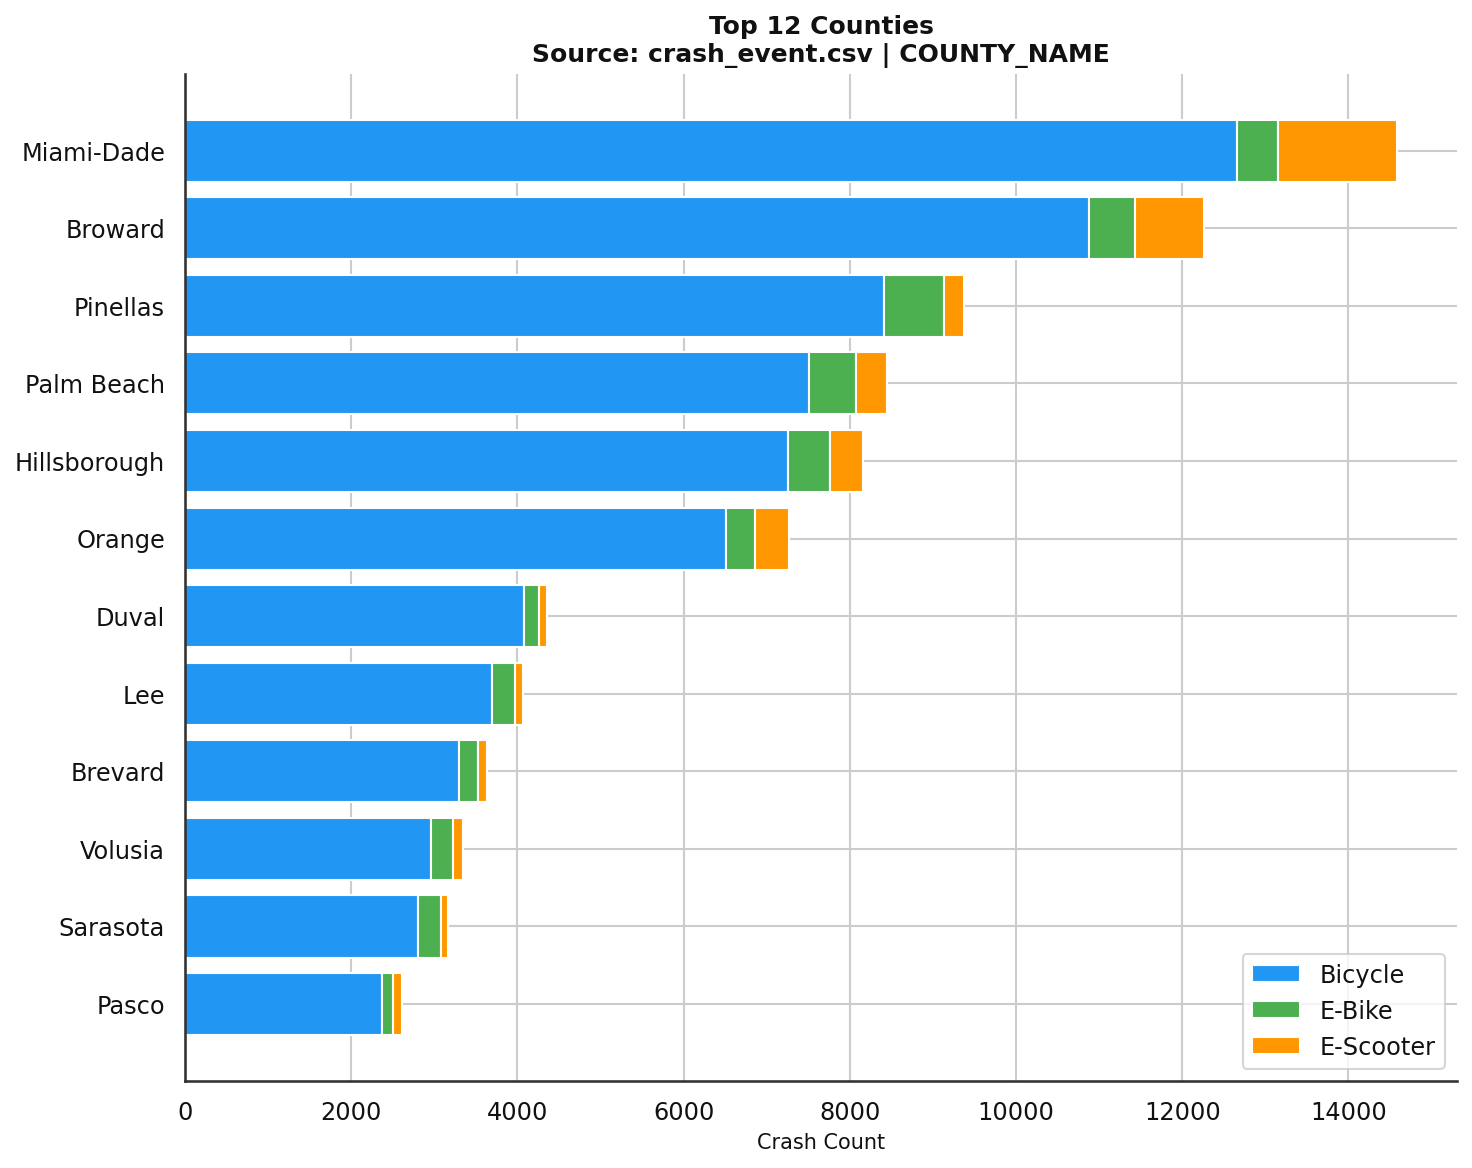
\includegraphics[width=0.9\linewidth,height=12.5cm,keepaspectratio]{figures/4d_top_counties.png}
  \caption{Top 12 counties by crash count. E-scooter crashes concentrate in Miami-Dade and Broward; e-bike crashes lead in Pinellas and Palm Beach.}
\end{figure}

  \end{block}

  \begin{block}{Limitations}
  \begin{itemize}
    \item E-bike and e-scooter counts are a \textcolor{posterblue}{\textbf{floor}}: a crash is recovered only if the officer names the device.
    \item There is \textcolor{posterblue}{\textbf{no exposure data}} (trips or miles), so shares describe crashes, not risk per trip.
    \item Mode labels agree strongly with the coded mode ($\kappa$ = 0.89), but LLM fault labels agree only modestly with police crash typing ($\kappa$ = 0.33). 2026 is a partial year.
  \end{itemize}
  \end{block}

\end{column}

\separatorcolumn

\begin{column}{\colwidth}

\begin{figure}
  \centering
  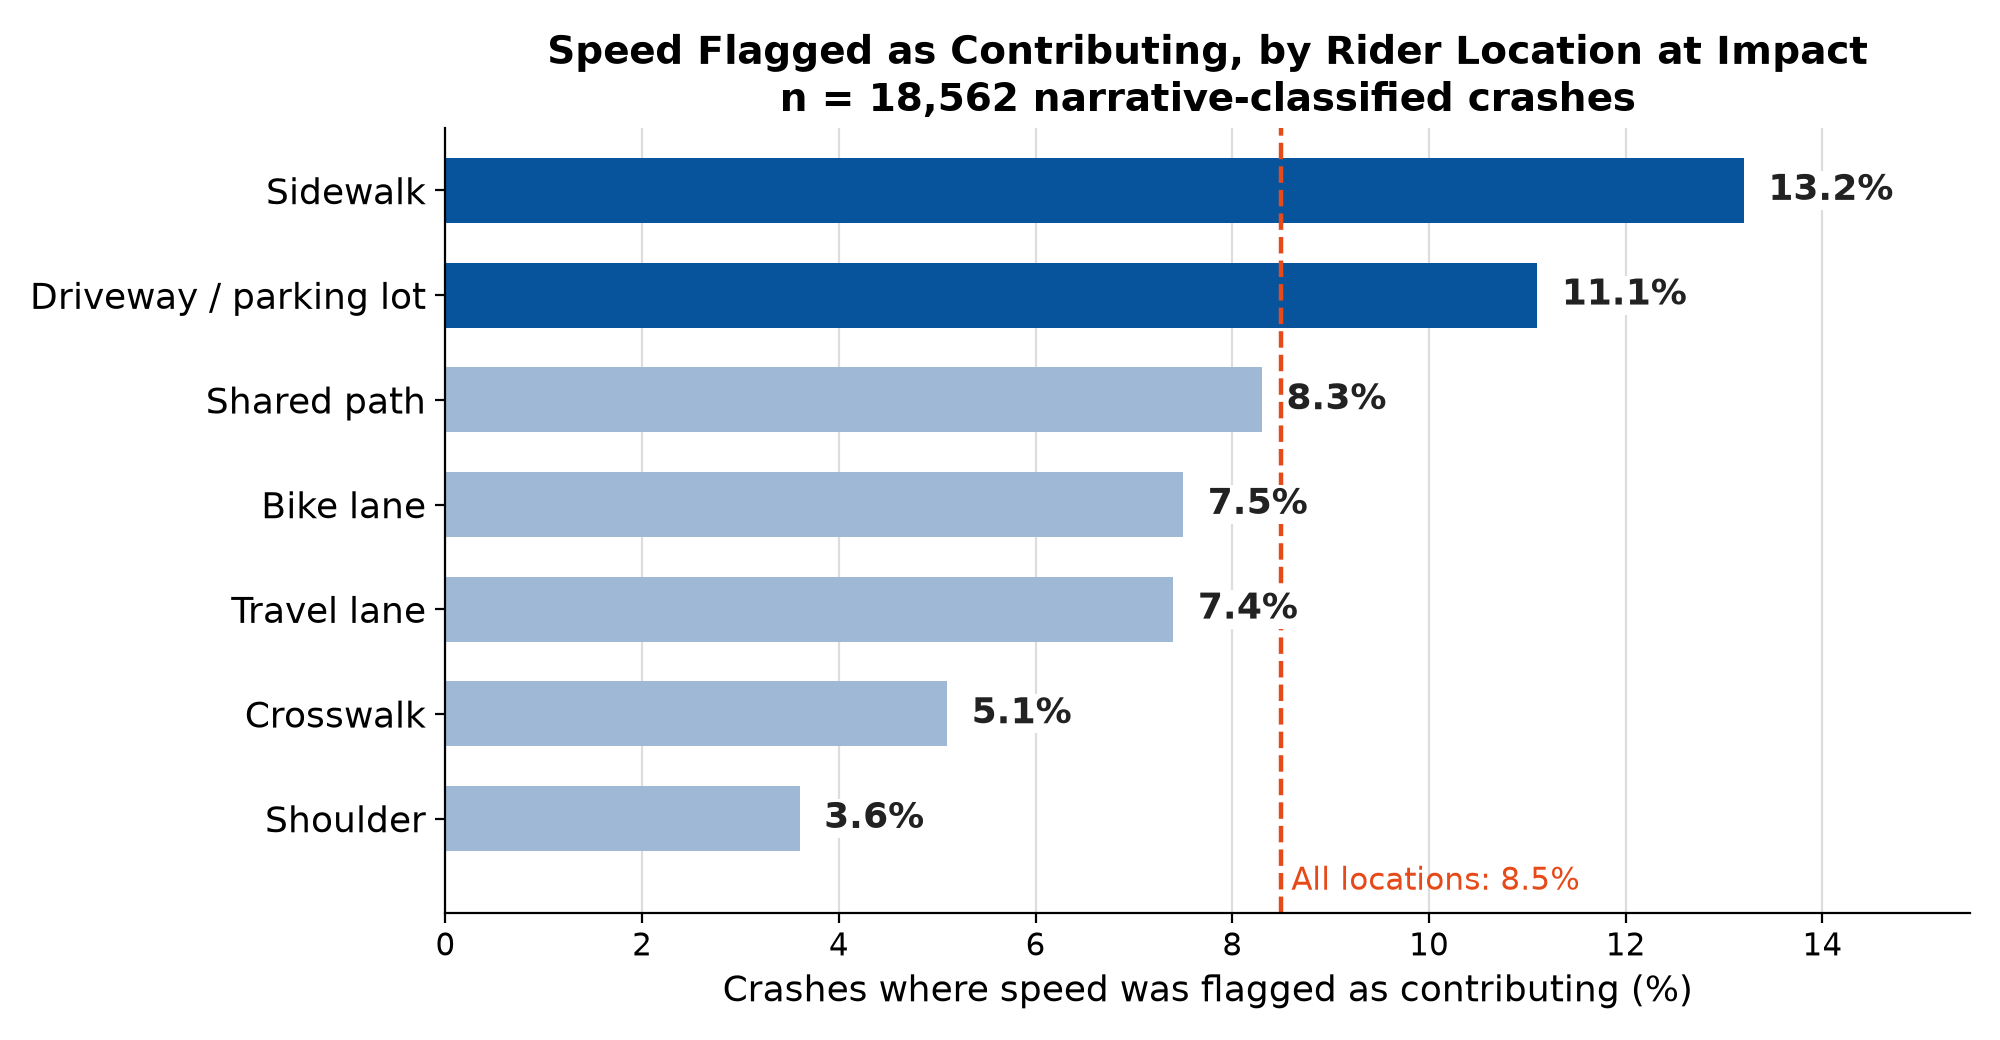
\includegraphics[width=\linewidth,height=15cm,keepaspectratio]{figures/speed_by_location.png}
  \captionsetup{font={small,bf,stretch=1.2}}
  \caption{Speed is flagged most often on sidewalks and at driveways, where riders cross paths with turning vehicles.}
\end{figure}

    \begin{alertblock}{Key findings}
    \begin{itemize}
      \item \textcolor{posterorange}{\textbf{Different riders.}} E-scooter riders are the youngest (median 26 vs. 33 for e-bikes and 38 for bicycles) and the most often female (31\% vs. 18--20\%).
      \item \textcolor{posterorange}{\textbf{Electric is not more severe.}} Fatal shares are 2.1\%, 1.4\%, and 1.3\%. The risk factors are \textcolor{posterorange}{\textbf{night}} (fatal 2.2--2.5$\times$ as often as overall) and \textcolor{posterorange}{\textbf{rider age}} (65+ die 4.9$\times$ as often as riders aged 18--24).
      \item \textcolor{posterorange}{\textbf{Few crashes are in bike lanes.}} Riders were on a sidewalk or crosswalk in 57.5\% of crashes and in a bike lane in 9.4\%. In bike lanes, 59.7\% involve a driver turning across the rider.
      \item \textcolor{posterorange}{\textbf{Speed is a powered-mode problem.}} Speed is flagged 4.6$\times$ as often for e-bikes and 2.5$\times$ for e-scooters as for bicycles. E-scooter crashes cluster in Miami-Dade, Broward, and all six major university counties (top 7 of 50 per capita).
    \end{itemize}
  \end{alertblock}

  \begin{block}{Countermeasures and future directions}
1. Add \textcolor{posterblue}{\textbf{e-bike (with class) and e-scooter fields}} to the Florida crash report; use LLM classification as a bridge.

2. Build \textcolor{posterblue}{\textbf{protected intersections}} at bike-lane crossings and treat sidewalk--driveway conflict points.

3. Manage \textcolor{posterblue}{\textbf{powered-device speed}} on sidewalks, with geofenced scooter caps near campuses and urban cores.

4. Target \textcolor{posterblue}{\textbf{night lighting}} and \textcolor{posterblue}{\textbf{older road users}}: an aging driver is flagged in 13.8--15.9\% of crashes, alcohol in 0.2--0.6\%.

5. Next: add \textcolor{posterblue}{\textbf{exposure data}} (trips or miles) to compare risk rates, and model injury severity by mode.
  \end{block}

\end{column}

\separatorcolumn
\end{columns}
\end{frame}

\end{document}
